% !TeX root = ../main.tex
\section{Controlled Verification Methodology}

\subsection{Experimental Objects}

The evaluation uses two controlled TypeScript/Node.js datasets. Dataset D1 is an end-to-end Order Platform benchmark whose expected baseline contains five components and five directed relationships. Twenty patches are distributed as nine no-impact changes, seven rule violations, and four architecture evolutions. In addition to refactoring, service bypass, required-edge removal, Redis, and AMQP cases from the initial benchmark, the expansion includes documentation-only URLs, type-only imports, method-name lookalikes, direct gateway database access, allow-rule violations, a broken multi-hop path, aliased PostgreSQL construction, a new service, and a Redis hash operation.

Each D1 case declares changed files, expected graph delta, classification, findings, and source location. The topology labels and classifications originated in Phase 1. Patch implementations and exact evidence lines were refined while the Phase 2 analyzer was integrated. D1 is therefore a development benchmark and regression oracle, not a blinded holdout. Validators check structural consistency, distribution, patch applicability, changed-file membership, patch-hunk containment, and integrity hashes; they do not replace independent semantic review.

Dataset D2 is a detector challenge corpus with five groups: \texttt{fetch}, PostgreSQL, Redis, AMQP publish, and AMQP consume. Each group contains four positive and four hard-negative source lines, giving 20 positives and 20 negatives. Positive variants include aliases, namespace imports, environment fallbacks, and multiple supported operations. Hard negatives include URL text without a call, custom functions, unused package imports, local objects with detector-shaped method names, lifecycle calls, comments, and string literals. The manifest binds each signal to a detector, source file, exact line, expected edge, description, and required source substring.

D2 was authored after the initial v0.1 analyzer and deliberately targets its weaknesses. We execute both the frozen v0.1 artifact and provenance-aware v0.2 on the same corpus. This paired comparison identifies concrete regression behavior but is not an unbiased estimate of improvement on unseen programs.

The Phase 3 protocol reuses D1 rather than introducing a third dataset. For each case, it creates a fresh Git repository from the unchanged baseline, commits that baseline with fixed author metadata, applies one patch to the working tree, and runs the diff gate twice. The first execution reconstructs and caches the base graph; the second must hit the cache. A separate full scan of the same patched head acts as an equivalence oracle for the incremental result. Ground truth is extended operationally with expected changed files and the PASS/BLOCK/REVIEW mapping already implied by each D1 label. We compare normalized cold and warm results, decisions, changed-file sets, exact architecture deltas, rule identifiers, evidence locations, and incremental/full-scan equivalence. Timings are retained only from the recorded Windows run because shared CI runners do not provide a controlled performance environment.

Figure~\ref{fig:evaluation-protocol} summarizes the executable verification protocol and shows how raw analyzer executions become the reported metrics and evidence artifact.

\subsection{External-Comparison Boundary}

External comparison remains future work; it was not executed within the reported evaluation. No accepted comparator result or common label mapping is available. A module-dependency analyzer is a candidate because it can express constraints on static dependencies in JavaScript/TypeScript, but selecting a tool does not establish equivalence between its observations and ArchSync's typed service relationships. That equivalence must be defined and reviewed before comparative measurements are interpreted.

The proposed comparison must distinguish the unit being labeled, the relationship a detector can observe, and the architecture rule applied to that relationship. A module import and a remote service call may occur in the same file without describing the same architecture edge. Conversely, a common abstraction may be possible if independently authored labels specify how both observations map to it. No common label mapping has been established. Unsupported HTTP, database, cache, or messaging relationships must not automatically become comparator false negatives.

The proposed protocol requires freezing repositories and revisions, tool versions and configurations, dependency-resolution conditions, independently reviewed ground truth, and the common scoring unit before inspecting outputs. It should record unsupported cases separately from misses within supported scope. The proposed protocol rejects a comparator unless a non-empty semantic intersection is established; any adapter must be separately frozen before execution. A qualitative capability discussion cannot complete that baseline or support precision, recall, or superiority claims. Reusing D1 would still evaluate author-developed examples; independent data would be needed to address the holdout limitation. These requirements describe planned work and contribute no executions or observations to the results below.

\begin{figure*}[t]
  \centering
  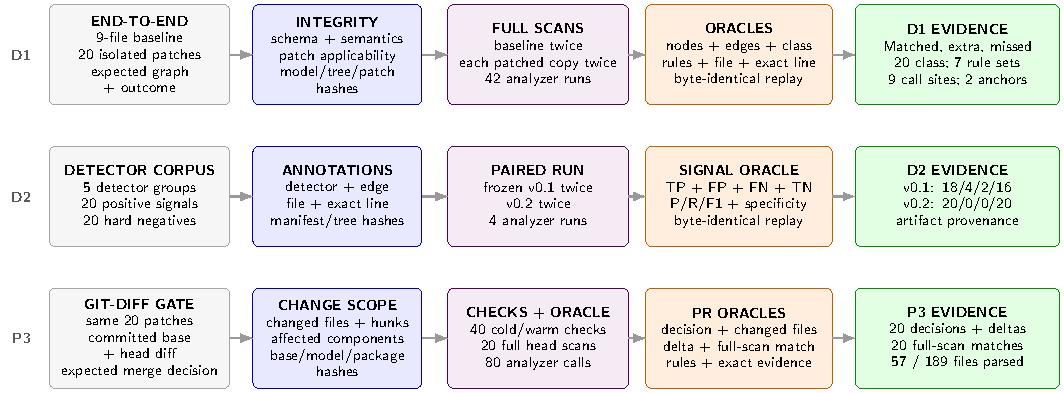
\includegraphics[width=\textwidth]{figures/Fig-2.pdf}
  \caption{Controlled verification protocol. D1 measures full-repository reconstruction and classification, D2 isolates detector signals, and P3 replays D1 as cold and warm Git-diff pull-request checks. All three routes use co-developed development data.}
  \Description{The first route validates 20 isolated executable patches and compares graphs, classifications, rules, evidence, and replay. The second validates 40 detector signals with two analyzer versions. The third commits the same baseline, applies each patch as a Git diff, performs cold and warm checks plus a full head scan, and measures decisions, changed files, architecture deltas, incremental equivalence, cache behavior, scope, evidence, and latency.}
  \label{fig:evaluation-protocol}
\end{figure*}

\subsection{Procedure}

The executed procedure for D1 was:
\begin{enumerate}
  \item validate the expected architecture, ground-truth manifest, hashes, and all patch applications;
  \item analyze the unchanged baseline twice;
  \item for each case, copy the baseline into a fresh temporary directory and apply exactly one patch;
  \item analyze the patched repository twice;
  \item compare predicted nodes, edges, classification, violated rule identifiers, and source evidence with ground truth; and
  \item remove the temporary directory before the next case.
\end{enumerate}

D1 performs 42 analyzer executions: two for the baseline and two for each of 20 cases. For D2, the manifest and annotated lines are validated before the entire repository is analyzed twice with each pinned analyzer version. Each observed relationship is expanded into detector--edge--file--line signals and compared with the annotations. D2 therefore adds four recorded executions, 46 across the reported current and historical Phase 2 evidence. The continuously rerun v0.2 gate executes 44 of them and verifies the frozen v0.1 package without rewriting that historical result.

P3 performs 40 change-scoped checks, one cold and one warm per case. Each cold check invokes a full baseline analysis and an affected-component analysis; each warm check reuses the baseline cache and invokes only the affected-component analysis. An additional full head scan per case verifies the incremental result, giving 80 analyzer calls. The normalized results compared across cold and warm runs exclude elapsed time and cache-hit state but retain changed files, affected components, graph delta, findings, evidence, and scan scope. The oracle must match head classification, decision, finding set, graph delta, and scanned-file count.

Repeated results are compared as normalized JSON. The benchmark workflow installs SHA-256-verified runtime packages and executes the Phase 2 and Phase 3 protocols plus the PASS/BLOCK/REVIEW quickstart from clean \texttt{ubuntu-latest} and \texttt{windows-latest} checkouts; both jobs passed for benchmark audit commit \texttt{5fe3679}.

\subsection{Metrics}

D1 reports counts of matched, extra, and missed graph items, with changed items separated from repeated baseline structure. For D2 only, TP and FN count annotated positive detector signals, and TN and FP count explicitly annotated hard negatives. Its descriptive precision, recall, F1, and specificity are
\begin{align}
  \operatorname{Precision} &= \frac{TP}{TP+FP},\\
  \operatorname{Recall} &= \frac{TP}{TP+FN},\\
  F_1 &= 2\cdot\frac{\operatorname{Precision}\cdot\operatorname{Recall}}
  {\operatorname{Precision}+\operatorname{Recall}},\\
  \operatorname{Specificity} &= \frac{TN}{TN+FP}.
\end{align}
We report both complete-graph and patch-changed node and edge counts. When both expected and predicted changed sets are empty, the case is an exact match but contributes no positive item to the aggregate TP/FP/FN counts. D2's TP, FP, FN, and TN units are annotated detector signals rather than distinct graph edges; several positive source locations may support the same edge.

Classification agreement is measured across all 20 cases. Rule-set agreement is measured on the seven violation cases. File and exact-line agreement are measured on the 11 finding-bearing cases; exact-line agreement means that at least one evidence item for the matched finding has the expected file and line. Determinism requires byte-identical normalized output across duplicate executions.

P3 additionally measures exact merge-decision, changed-file-set, architecture-delta, and incremental/full-scan agreement. Incremental scope is
\begin{equation}
  r_{\mathrm{parse}}=\frac{\sum_i |T_i^{\mathrm{parsed}}|}{\sum_i |T_i^{\mathrm{head}}|},
\end{equation}
where $T_i^{\mathrm{parsed}}$ contains TypeScript files parsed in affected components and $T_i^{\mathrm{head}}$ contains TypeScript files represented by the reconstructed head graph. Cache correctness requires a miss followed by a hit for every isolated case and identical normalized results. Cold and warm check latency are summarized by median and 95th percentile; no inferential comparison is made.

\subsection{Engineering Acceptance Criteria}

Before reporting the controlled run, the D1 engineering exit gate required node and edge precision and recall of at least 0.85 for both complete and changed graphs, exact classification for every case, exact violated-rule sets, matching evidence files and lines, deterministic replay, and repository-specific coverage thresholds. D2 v0.2 additionally required zero missed positive signals, zero unexpected detections, all 20 hard negatives rejected, and byte-identical replay. P3 required exact classification, decision, changed-file sets, architecture deltas, rule sets, source files and lines for all applicable cases; full-scan equivalence, cache hits, and identical normalized replay for all repeated checks; and cross-platform completion of the full benchmark workflow. The value 0.85 is an engineering prototype threshold rather than a statistically derived standard. Passing these criteria verifies the declared regression contract only; it does not establish superiority to an external tool or accuracy on unseen repositories.
